\subsection{Operating point for t<0}
For t<0, from equation (por aqui equação da função de ramos da voltagem) we can see that $v_s (t)= V_s$. That means the voltage source drives constant voltage $V_s$. We consider that enough time has passed for the capacitor to fully charge from this constant voltage, so the voltage at nodes 6 and 8 are the same and there is no current flowing through the capacitor (it now acts as an open circuit). Removing the part of the circuit that is an open circuit we get a "new" circuit, that is easy to analyse: \\
\begin{figure}[h] \centering
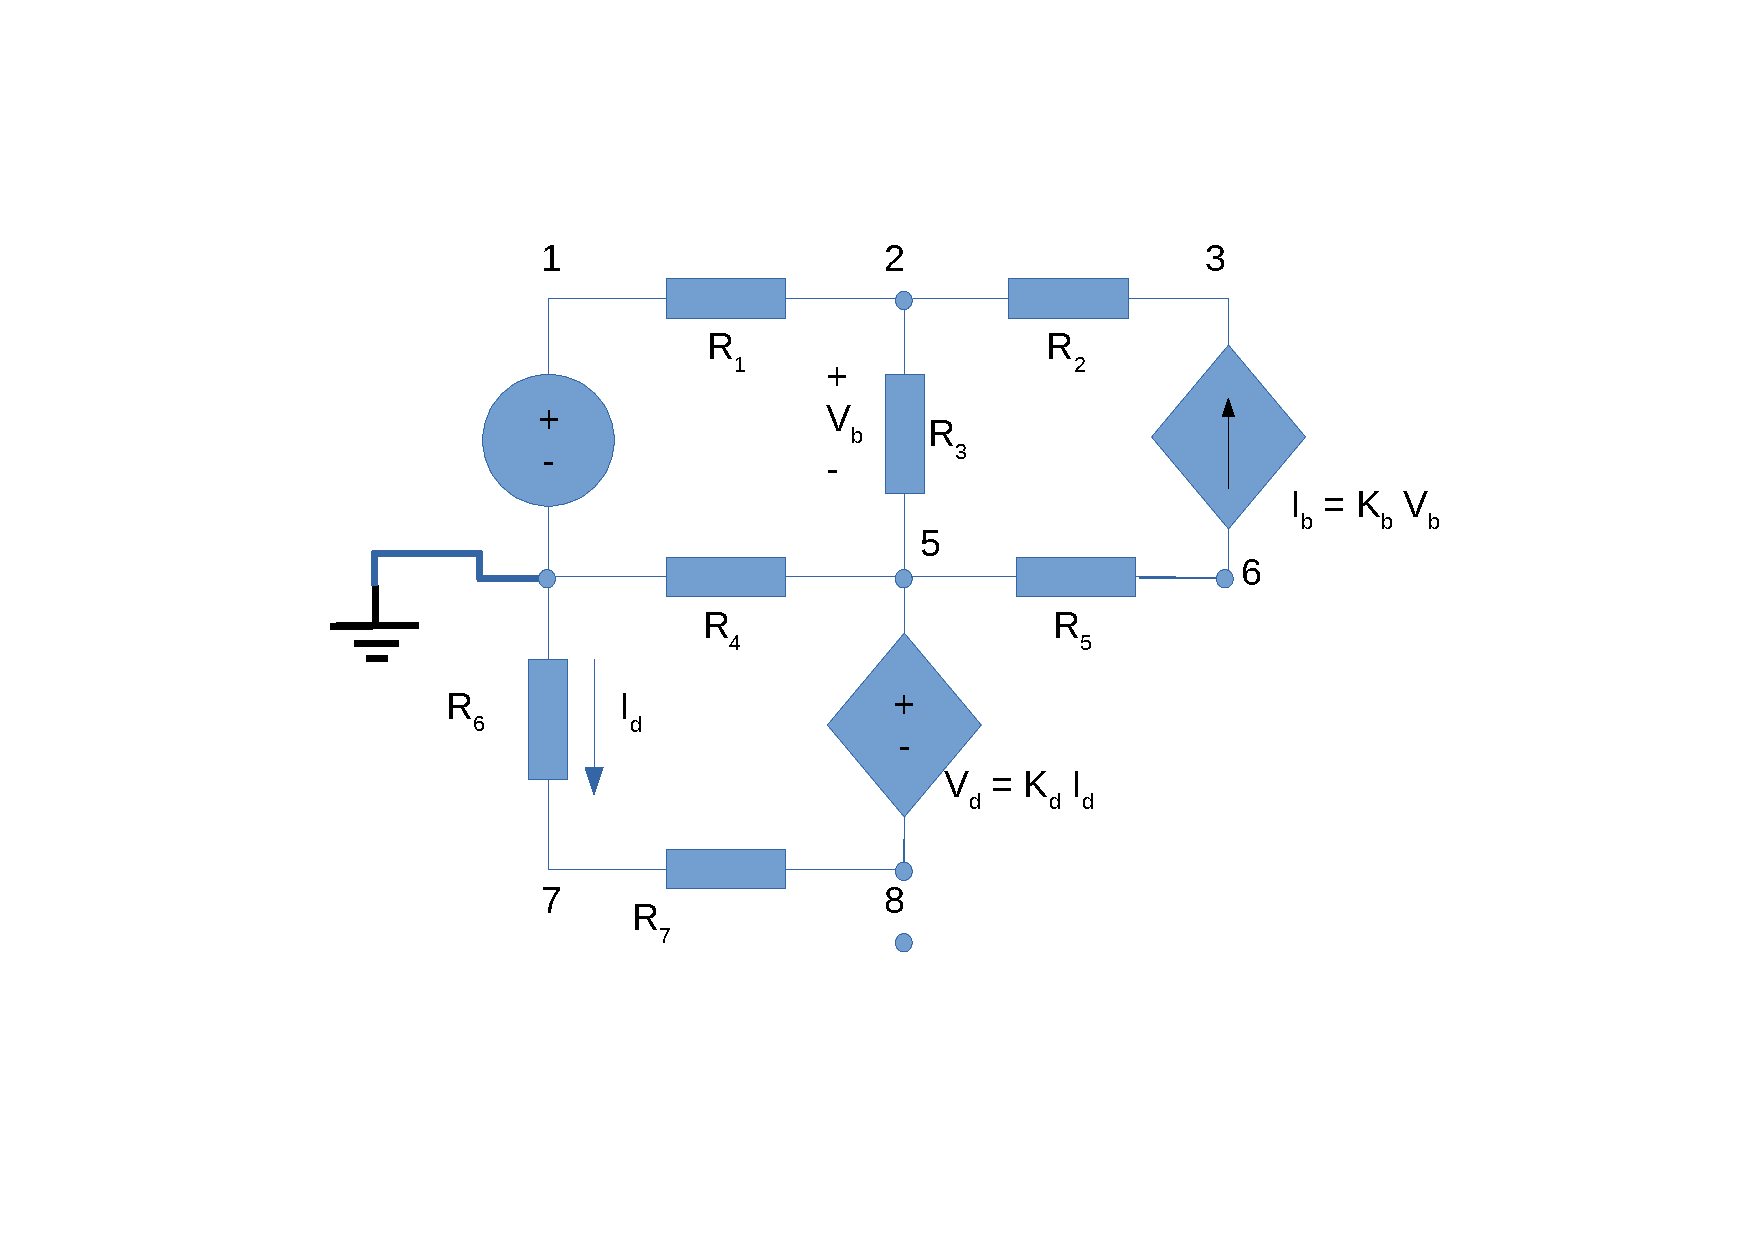
\includegraphics[width=0.8\linewidth]{tmenor0.pdf}
\caption{Circuit to analyse for t<0}
\label{fig:zim}
\end{figure}

In this circuit, there are 8 nodes, one of which is a ground node (the one that connects $R_4$, the voltage source and $R_6$. Therefore, to solve the circuit we must find 7 independent equations. \\
To discover the equations for each node we need to use Kirchhoff’s Current Law, which states that the sum of all the currents entering and leaving a node must be equal to zero. For simplicity instead of using directly the currents we will also use Ohm's Law and we will consider that all currents are leaving the nodes. \\
The equations for the 7 nodes are:
\begin{equation}
    V_{1}=V_{s} 
\end{equation}
\begin{equation}
  \frac{V_{2}-V_{1}}{R_{1}} +\frac{V_{2}-V_{3}}{R_{2}}+\frac{V_{2}-V_{5}}{R_{3}}=0 
\end{equation}
\begin{equation}
  V_{5}-V_{2}+\frac{V_{3}-V_{2}}{R_{2} K_b}=0
\end{equation}
\begin{equation}
   \frac{V_{5}}{R_{4}} + \frac{V_{5}-V_{6}}{R_{5}}+ \frac{V_{8}-V_{7}}{R_{7}} + \frac{V_{5}-V_{2}}{R_{3}}=0 
\end{equation}
\begin{equation}
    \frac{V_{3}- V_{2}}{R_{2}} + \frac{V_{6}-V_{5}}{R_{5}} = 0
\end{equation}
\begin{equation}
    V_{7}+ R_6 \left(\frac{V_{7}-V_{8}}{R_{7}}\right) = 0
\end{equation}
\begin{equation}
  V_{8}-V_{5} + K_d \left(\frac{V_{8}-V_{7}}{R_{7}}\right) = 0
\end{equation}
\\
The next step is to solve the system of equations: \\
\\
\left(\begin{array}{ccccccc} 
1 & 0 & 0 & 0 & 0 & 0 & 0\\
-\frac{1}{R_1} & \frac{1}{R_1}+\frac{1}{R_2}+\frac{1}{R_3} & -\frac{1}{R_2} & -\frac{1}{R_3}& 0 & 0 & 0 \\
0 & -1-\frac{1}{R_2 K_b} & \frac{1}{R_2 K_b} & 1 & 0 & 0 & 0 \\
0 & -\frac{1}{R_3} & 0 & \frac{1}{R_3} +\frac{1}{R_4}+\frac{1}{R_5} & -\frac{1}{R_5} & -\frac{1}{R_7} & \frac{1}{R_7} \\
0 & -\frac{1}{R_2} & \frac{1}{R_2} & -\frac{1}{R_5} & \frac{1}{R_5} & 0 & 0 \\
0 & 0 & 0 & 0 & 0 & 1+\frac{R_6}{R_7} & -\frac{R_6}{R_7} \\
0 & 0 & 0 & -1 & 0 & -\frac{K_d}{R_7} & 1 + \frac{K_d}{R_7} \\
\end{array}\right)
\left(\begin{array}{c} V_1 \\ V_2 \\ V_3 \\ V_5 \\ V_6 \\ V_7 \\ V_8 \end{array}\right) 
= \left(\begin{array}{c} V_s\\ 0 \\ 0 \\ 0 \\0 \\ 0 \\0 \end{array}\right)
